\chapter{EASI Library Architecture Deep-Dive}
\label{sec:appendix_architecture}

\section{Process Flow}
\label{sec:appendix_process}

Figure~\ref{fig:process_flow} shows the full lifecycle of an \texttt{easi start} invocation, from CLI parsing through episode execution to final cleanup. Component interactions proceed top-to-bottom; the subprocess boundary separates the host process from simulator bridge processes.


\begin{figure}[htbp]
\centering
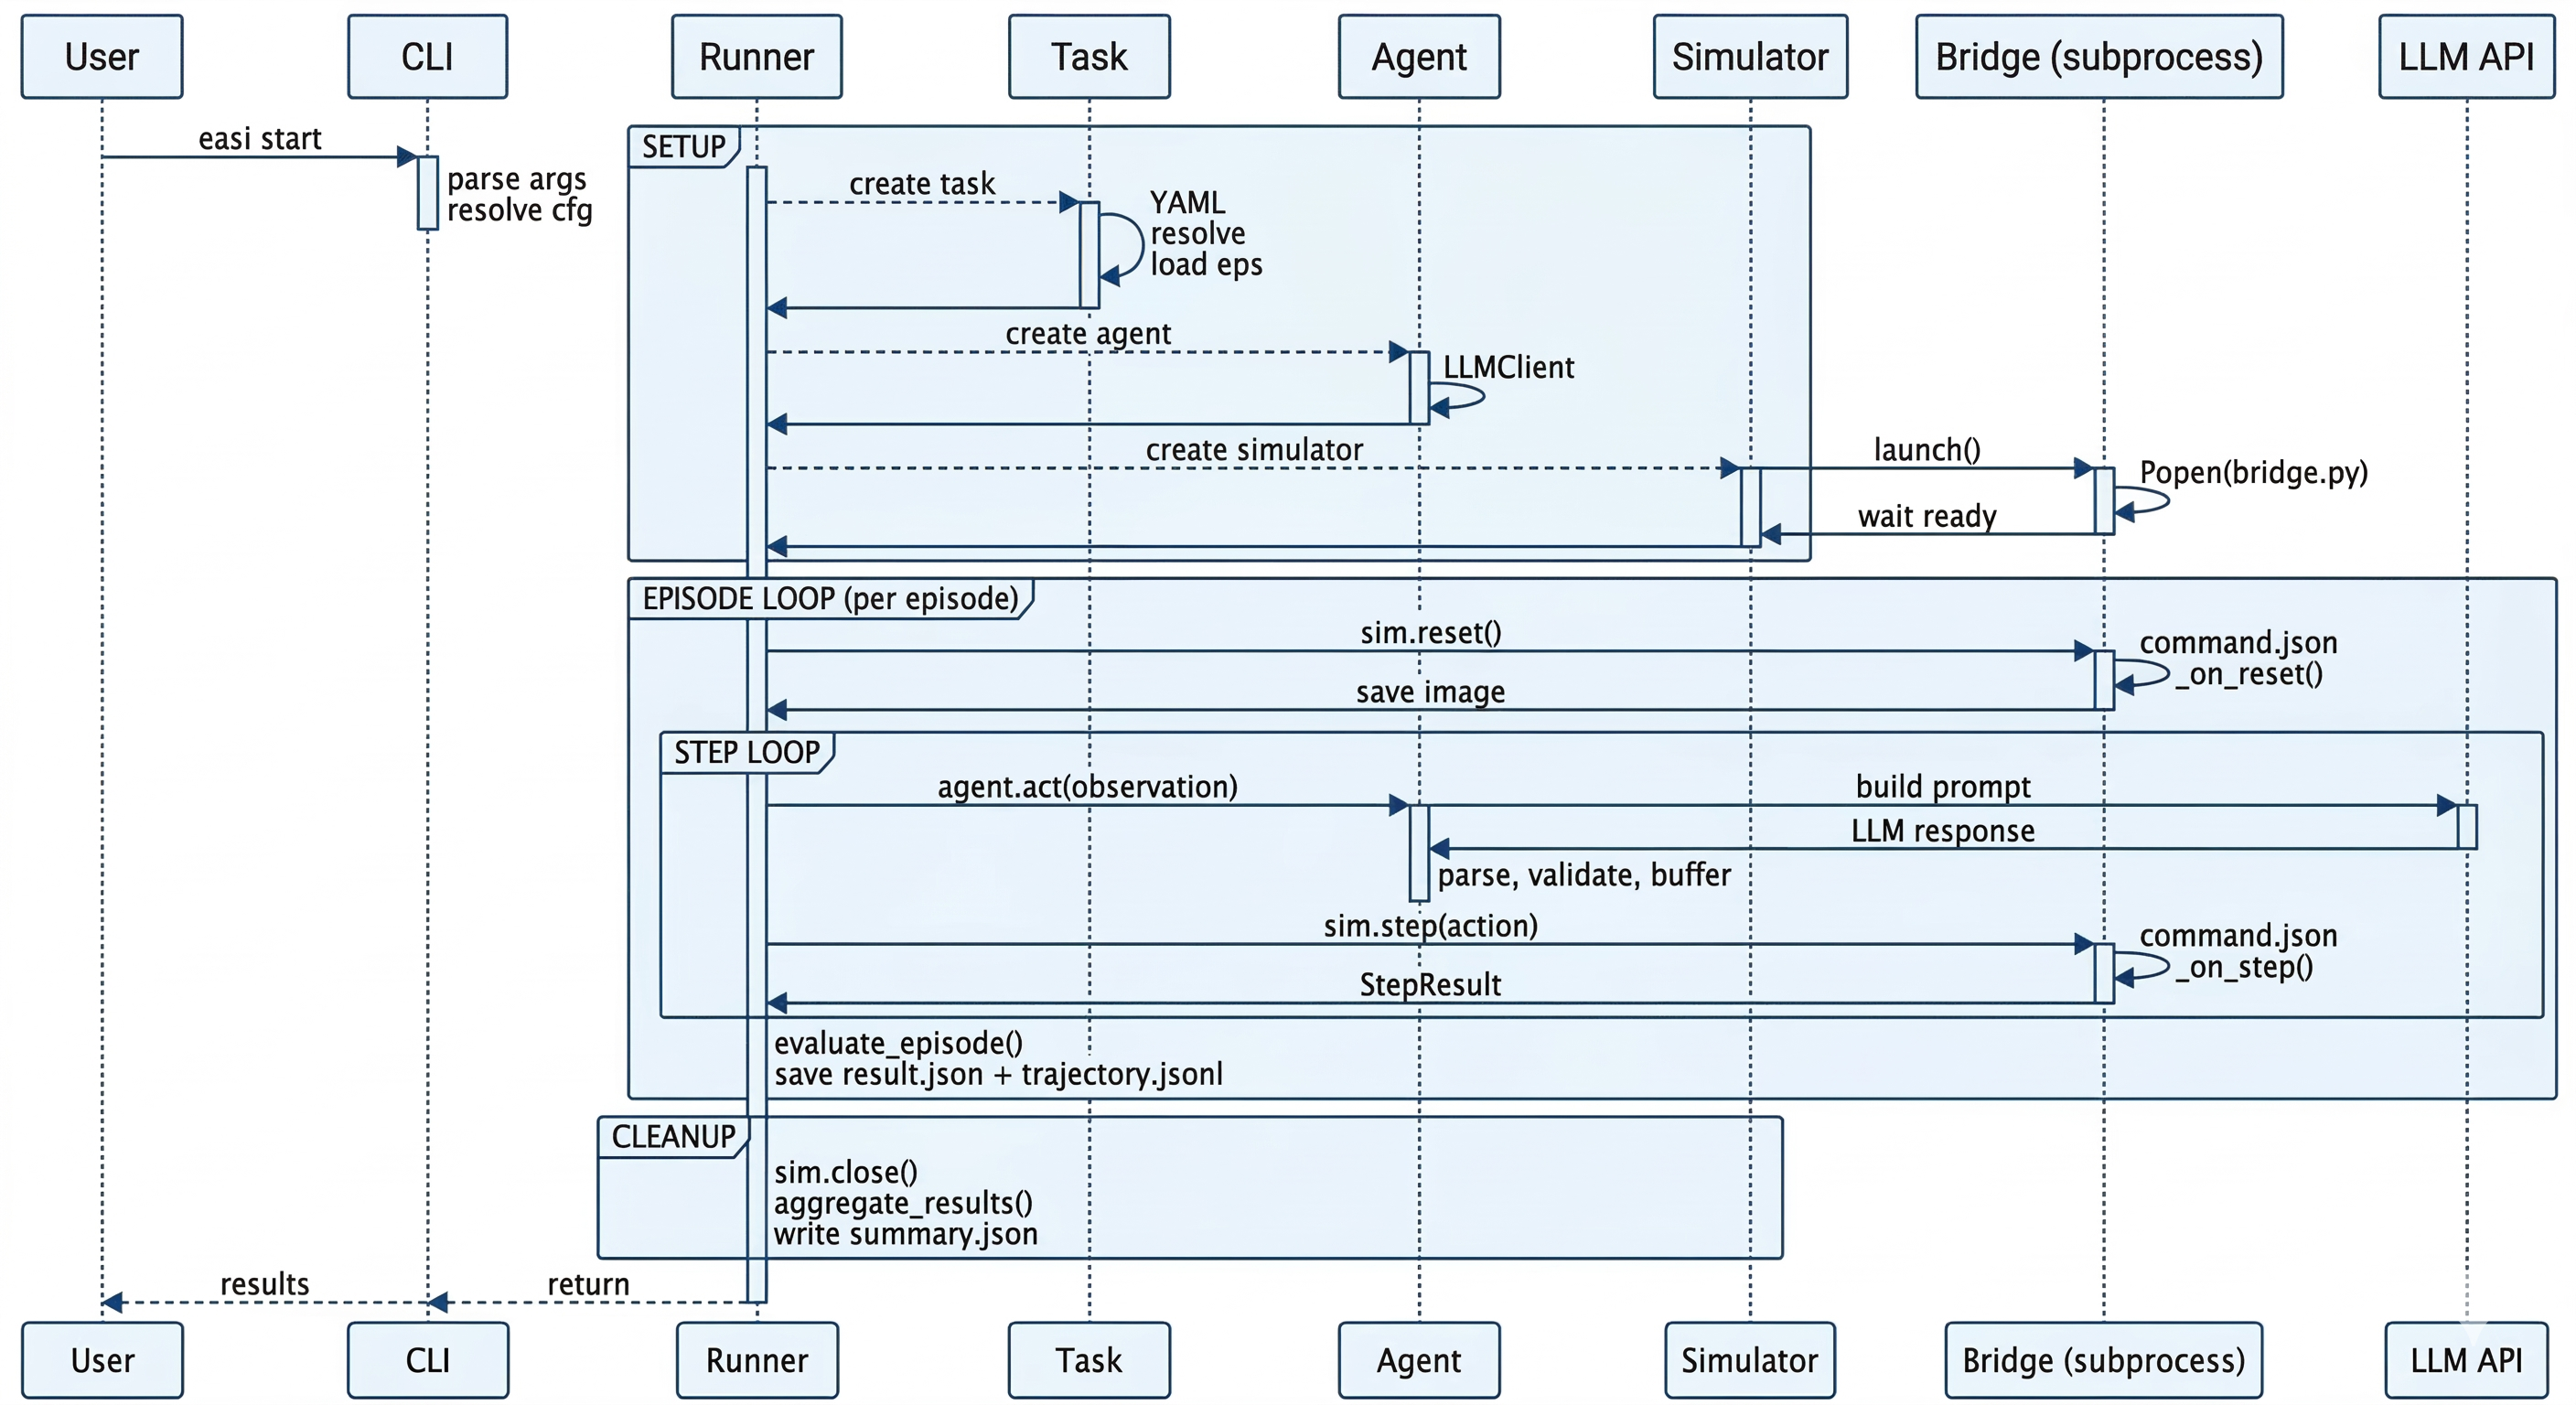
\includegraphics[width=\textwidth]{fig/process_flow.png}
\caption{Sequence diagram showing the full lifecycle of an \texttt{easi start} invocation.}
\label{fig:process_flow}
\end{figure}

\section{IPC Protocol}
\label{sec:appendix_ipc}

Communication between the host process and each simulator bridge uses three JSON files in a temporary workspace directory:

\begin{lstlisting}[basicstyle=\ttfamily\small, numbers=none, backgroundcolor=\color{white}, frame=single]
/tmp/easi_XXXXXXXX/
  status.json       <- bridge writes on startup: {"ready": true}
  command.json      <- parent writes, bridge reads
  response.json     <- bridge writes, parent reads
\end{lstlisting}

All writes use an \textbf{atomic rename} pattern (\texttt{file.tmp} $\to$ \texttt{file.json}) to prevent partial reads. The parent polls \texttt{response.json} with a configurable interval (default 0.1s) and timeout, checking subprocess liveness on each poll. The supported command types are summarised in Table~\ref{tab:ipc_commands}.

\begin{table}[htbp]
\centering
\caption{IPC command types between the parent process and simulator bridge.}
\label{tab:ipc_commands}
\small
\renewcommand{\arraystretch}{1.1}
\begin{tabular}{llll}
\toprule
\textbf{Type} & \textbf{Parent Sends} & \textbf{Bridge Does} & \textbf{Bridge Returns} \\
\midrule
\texttt{reset} & episode\_id, config & Create/reset env & observation, reward, done \\
\texttt{step} & action\_name, params & Execute action & observation, reward, done \\
\texttt{close} & type: ``close'' & Cleanup, exit & status: ``ok'' \\
\bottomrule
\end{tabular}
\end{table}

\begin{table}[htbp]
\centering
\caption{EASI library component map (30+ modules organised by architectural layer).}
\label{tab:component_map}
\small
\renewcommand{\arraystretch}{1.1}
\begin{tabular}{lp{3.5cm}p{4cm}}
\toprule
\textbf{Layer} & \textbf{Components} & \textbf{Role} \\
\midrule
CLI \& Orchestration & \texttt{cli.py}, Runners, EpisodeFilter, Metrics & Parse args, manage episode loop, aggregate \\
Tasks & TaskRegistry, yaml\_utils, Dataset, BaseTask & Auto-discover, YAML inheritance, load datasets \\
Agents & ReActAgent, AgentMemory, PromptBuilder & LLM decisions, state tracking, prompt assembly \\
LLM & LLMClient, ServerManager, DummyServer & Unified LLM interface, vLLM lifecycle \\
Simulators & SimulatorRegistry, SubprocessRunner, BaseBridge & Auto-discover, IPC, process lifecycle \\
Communication & filesystem.py, schemas.py & Atomic JSON I/O, schemas \\
Rendering & RenderPlatform, XorgManager, Adapters & Display backend, Xorg servers, adjustments \\
Analysis & TrajectoryVideo, ProgressBar & Post-hoc video, progress display \\
\bottomrule
\end{tabular}
\end{table}

\section{Parallel Execution and Resource Management}
\label{sec:appendix_parallel}

The \texttt{ParallelRunner} extends the sequential runner with thread-pool concurrency. Each worker is fully isolated with its own simulator process, agent instance, and LLM client.

\begin{figure}[htbp]
\centering
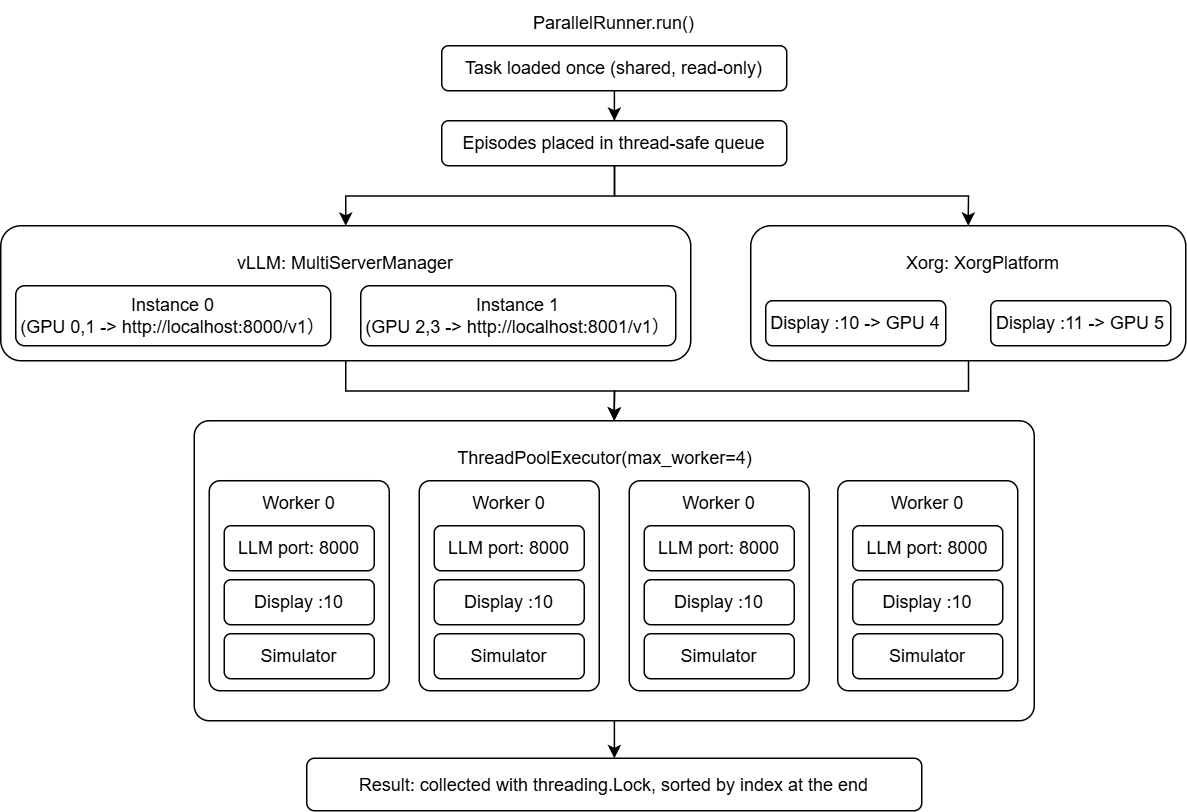
\includegraphics[width=\textwidth]{fig/parallel_flow.png}
\caption{ParallelRunner execution flow with thread-pool concurrency, multi-instance vLLM, and Xorg display management.}
\label{fig:parallel_flow}
\end{figure}

Resource assignment uses round-robin allocation:
\begin{itemize}
    \item LLM URLs: \texttt{base\_urls[worker\_id \% len(base\_urls)]} distributes workers evenly across vLLM instances
    \item GPU/display binding: \texttt{platform.for\_worker(worker\_id)} cycles through available render instances
    \item Thread-safe results: \texttt{threading.Lock} guards the shared results list
\end{itemize}

\begin{table}[htbp]
\centering
\caption{Render platform hierarchy and use cases.}
\label{tab:render_platforms}
\small
\renewcommand{\arraystretch}{1.1}
\begin{tabular}{llll}
\toprule
\textbf{Platform} & \textbf{Display} & \textbf{GPU Binding} & \textbf{Use Case} \\
\midrule
\texttt{auto} & Detect; fallback xvfb & Manual & Default \\
\texttt{native} & Existing \texttt{\$DISPLAY} & Manual & Desktop with X \\
\texttt{xvfb} & Virtual framebuffer & Manual & Headless (CPU) \\
\texttt{egl} & None (headless) & CUDA\_VISIBLE & GPU headless \\
\texttt{headless} & None & Manual & Native headless \\
\texttt{xorg} & \texttt{:N} per GPU & Auto-managed & GPU X11 \\
\bottomrule
\end{tabular}
\end{table}


\chapter{Prompt Format and Full Example}
\label{sec:appendix_prompt}

\section{Prompt Format Specification}

The EASI standard prompt format defines how the agent communicates with any LLM backend. It applies to all benchmarks that do not have a published prompt format (EmbodiedBench benchmarks retain their original formats for reproducibility). The system prompt follows a fixed section order as shown in Table~\ref{tab:prompt_sections}.

\begin{table}[htbp]
\centering
\caption{System prompt sections and their purposes.}
\label{tab:prompt_sections}
\small
\renewcommand{\arraystretch}{1.1}
\begin{tabular}{lcp{5cm}}
\toprule
\textbf{Section} & \textbf{Req.} & \textbf{Purpose} \\
\midrule
Role and Environment & Yes & Agent identity and environment \\
Observation Description & No & Non-visual feedback explanation \\
Available Actions & Yes & Action names, descriptions, params \\
Strategy & No & Benchmark-specific tactical advice \\
Guidelines & Yes & Universal rules \\
Response Format & Yes & The 4-field JSON schema \\
\bottomrule
\end{tabular}
\end{table}

The response follows a 4-field JSON schema as shown below.
\begin{lstlisting}[language=Java, basicstyle=\ttfamily\small, numbers=none]
{
    "visual_state_description": "Describe what you see",
    "reasoning_and_reflection": "Reason about situation",
    "language_plan": "Describe next plan",
    "executable_plan": [
        {"action": "move_forward"},
        {"action": "turn_left"}
    ]
}
\end{lstlisting}

The user message is assembled per step in the following order.
\begin{lstlisting}[basicstyle=\ttfamily\small, numbers=none, backgroundcolor=\color{white}, frame=single]
[Image(s)]                    <- base64 encoded
[Text content:]
  ## Task                     <- instruction
  ## Environment Feedback     <- current-step feedback
  ## Action History (last N)  <- compact action + outcome log
  ## Chat History (last N)    <- previous LLM responses
  [Response format reminder]  <- brief JSON format hint
\end{lstlisting}

\section{Complete Prompt Example: Navigation Episode}

The following shows the exact prompt sent to the LLM during step 5 of a VLN-CE navigation episode.

The system prompt for this episode is shown below.

\begin{lstlisting}[basicstyle=\ttfamily\small, numbers=none, backgroundcolor=\color{backcolour}]
## Role and Environment
You are a robot navigating in a 3D indoor environment.
You observe the environment through a front-facing camera
and must follow natural language instructions to navigate
to a goal location.

## Observation Description
- **Distance to goal**: Geodesic distance in meters to
  the goal. Decreases as you approach the destination.

## Available Actions
- move_forward: Move forward by 0.25 meters
- turn_left: Turn left by 15 degrees
- turn_right: Turn right by 15 degrees
- stop: Stop and end navigation (use ONLY when you
  believe you have reached the destination)

## Strategy
1. Carefully read the navigation instruction
2. Observe your surroundings in the image
3. Follow the instruction step by step
4. Use stop ONLY when confident you have reached
   the described destination

## Guidelines
1. Always output at least one action.
2. Only use actions from the Available Actions list.
3. If previous actions failed, try a different approach.
4. Do not repeatedly execute the same action sequence.
5. Keep your plan efficient and concise.

## Response Format
Output a JSON object with exactly these 4 fields:
{
    "visual_state_description": "...",
    "reasoning_and_reflection": "...",
    "language_plan": "...",
    "executable_plan": [{"action": "<action_name>"}]
}
\end{lstlisting}

The user message at step 5 is as follows.


\begin{lstlisting}[basicstyle=\ttfamily\small, numbers=none, backgroundcolor=\color{backcolour}]
[Image: base64 encoded current view]

## Task
Walk down the hallway and turn right into the bedroom.

## Environment Feedback
Distance to goal: 5.3m

## Action History (last 5 steps)
Step 0: move_forward -> Distance to goal: 8.2m
Step 1: move_forward -> Distance to goal: 7.9m
Step 2: move_forward -> Distance to goal: 7.6m
Step 3: turn_right -> Distance to goal: 7.6m
Step 4: move_forward -> Distance to goal: 7.3m

Respond with the JSON format specified above.
\end{lstlisting}
